%    JJJ    AA     CCCCCC KKK   K TTTTTT HH  HH EEEEEE BBBBBB UU  UU SSSSSS    CCCCCC OOOOOO MM  MM
%    JJJ   AAAA    CCCCCC KKK  K  TTTTTT HH  HH EEEEEE BB   B UU  UU SSS       CCCCCC OOOOOO MM  MM
%    JJJ  AA  AA   CC     KKK K     TT   HHHHHH EEE    BB   B UU  UU SSS       CC     OO  OO MMMMMM
%    JJJ AA    AA  CC     KKKK      TT   HHHHHH EEEEEE BBBBBB UU  UU  SSSSS    CC     OO  OO M MM M
%    JJJ AAAAAAAA  CC     KKK K     TT   HH  HH EEE    BB   B UU  UU    SSS    CC     OO  OO M MM M
% JJJJJJ AA    AA  CCCCCC KKK  K    TT   HH  HH EEEEEE BB   B UUUUUU    SSS .. CCCCCC OOOOOO M MM M
% JJJJJJ AA    AA  CCCCCC KKK   K   TT   HH  HH EEEEEE BBBBBB UUUUUU SSSSSS .. CCCCCC OOOOOO M MM M
% 
% Texte Geschrieben von Stefan Bopp und Chantal Frunz
% Mehr Informationen sind auf jackthebus.com zu finden
%

\subsection{Freitag 06.04.2012}
Aus der geplanten frühen Abfahrt Richtung Zug wurde nichts.
Das Wetter zeigte sich leider eher von der bescheidenen Seite und so beschlossen wir das Ganze gemütlich anzugehen.
Den Einkauf habe ich schon am Vortage erledigt und auch Jack stand nach etlichen kleinen Ungereimtheiten wieder frisch da.
Die erste Überraschung gab es schon vor der Abfahrt.
Mein Fahrrad entschied sich die Luft des Pneus wieder der Umwelt zuzuführen.
Glücklicherweise steht im Keller noch ein zweites und der Umweg um es aufzuladen hält sich in Grenzen.
Die Fahrt verlief Ereignislos und schon bald konnten wir unsere Fahrräder satteln und eine kleine Tour um den See zu starten.
Es war zwar nicht gerade strahlender Sonnenschein aber trotzdem hielt sich das Wetter.
Der kurzfristige Wechsel des fahrbaren Drahtgestells führte dann auf dem Waldweg zu Herausforderungen, welche mit einem "`anständigen"' Velo so nicht zu meistern gewesen wären.
Nach einer kurzen Stärkung in Unterägeri schlossen wir die erfolgreiche Umrundung des Sees ab und begaben uns kurz nach 14 Uhr zum Campingplatz, welcher uns für die nächsten zwei Tage beherbergen sollte.

Da der Platz bei den mässigen Wettervorhersagen nicht gerade übervoll war, konnten wir uns einen Stellplatz aussuchen und positionierten uns in unmittelbare Nähe des Sees.
Als Nachbarn tauchten schon bald B.A Baracus und ein weiblicher Colonel John Smith mit einem genauen Imitat des bekannten Vans auf.
Unsere kleine mitgebrachte Heizung musste schon jetzt ihre Standfestigkeit unter Beweis stellen, da Chantal sich ohne Schlafsack nicht mehr aus dem aufgebauten Bett hervortraute.
Die zweite Büchse Chili con Carne, welche wir in Bonifacio letzten Sommer käuflich erworben haben, diente mir als willkommene Mahlzeit nach der kurzen Velotour.
Frisch gestärkt ging es an den Strand.
Sogar die Enten zog es an Land, die Temperaturen waren eher frostig. 
Nach dem Duschen, welches unerwartet unsere 50erli aufbrauchte, war es an der Zeit etwas zu kochen.
Die Temperaturen waren zwar tief, trotzdem entschieden wir uns vor dem Bus zu essen.
Nach dem obligaten Abwasch (der gerade Chantal immer wieder Spass macht) haben wir uns in den Bus verkrochen und unser Elektroöfeli das erste Mal so richtig gefordert.

\begin{figure}[H]
   \centering
      %\subfloat[CAPTION]{BILDERCODE}\qquad
   \subfloat{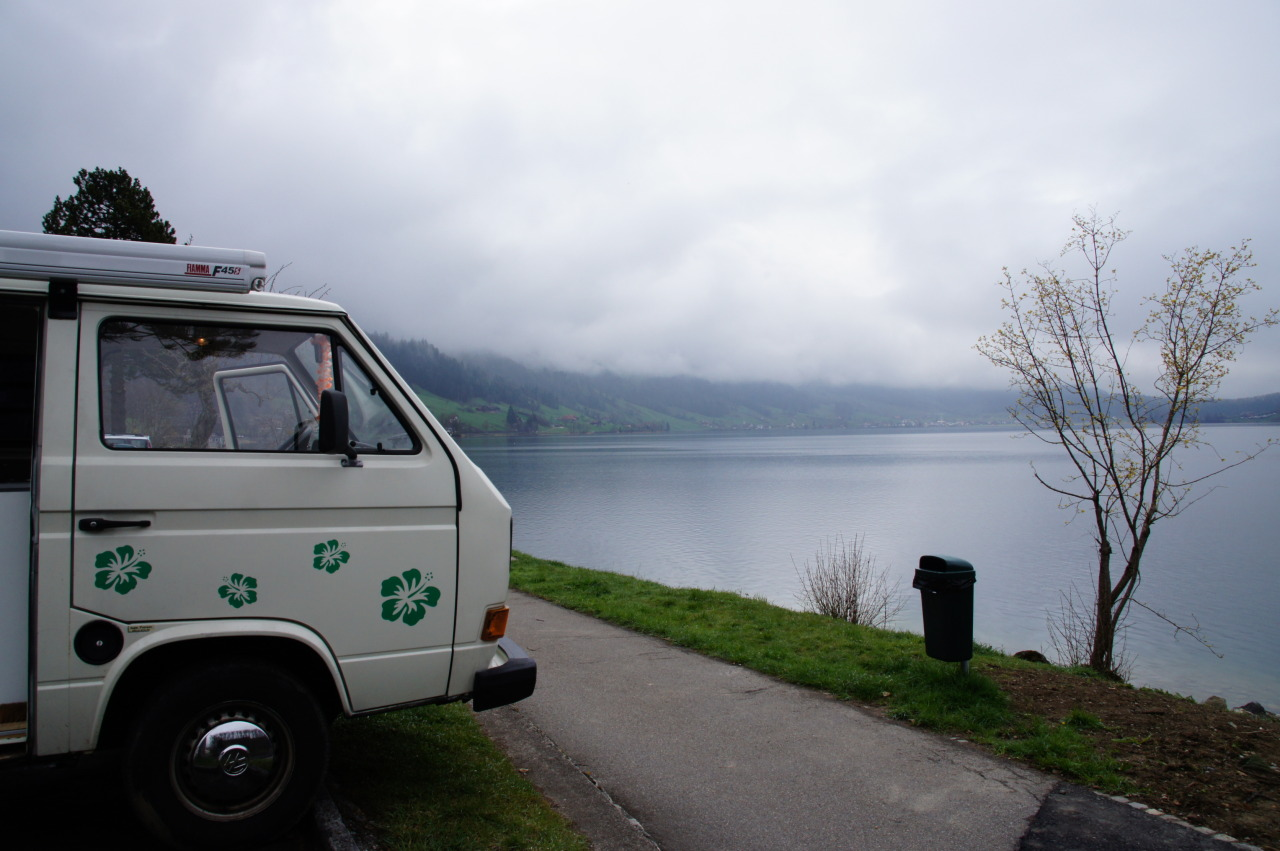
\includegraphics [width=0.3\textwidth]{../Bilder/Aegeri/1.jpg}}\quad
   \subfloat{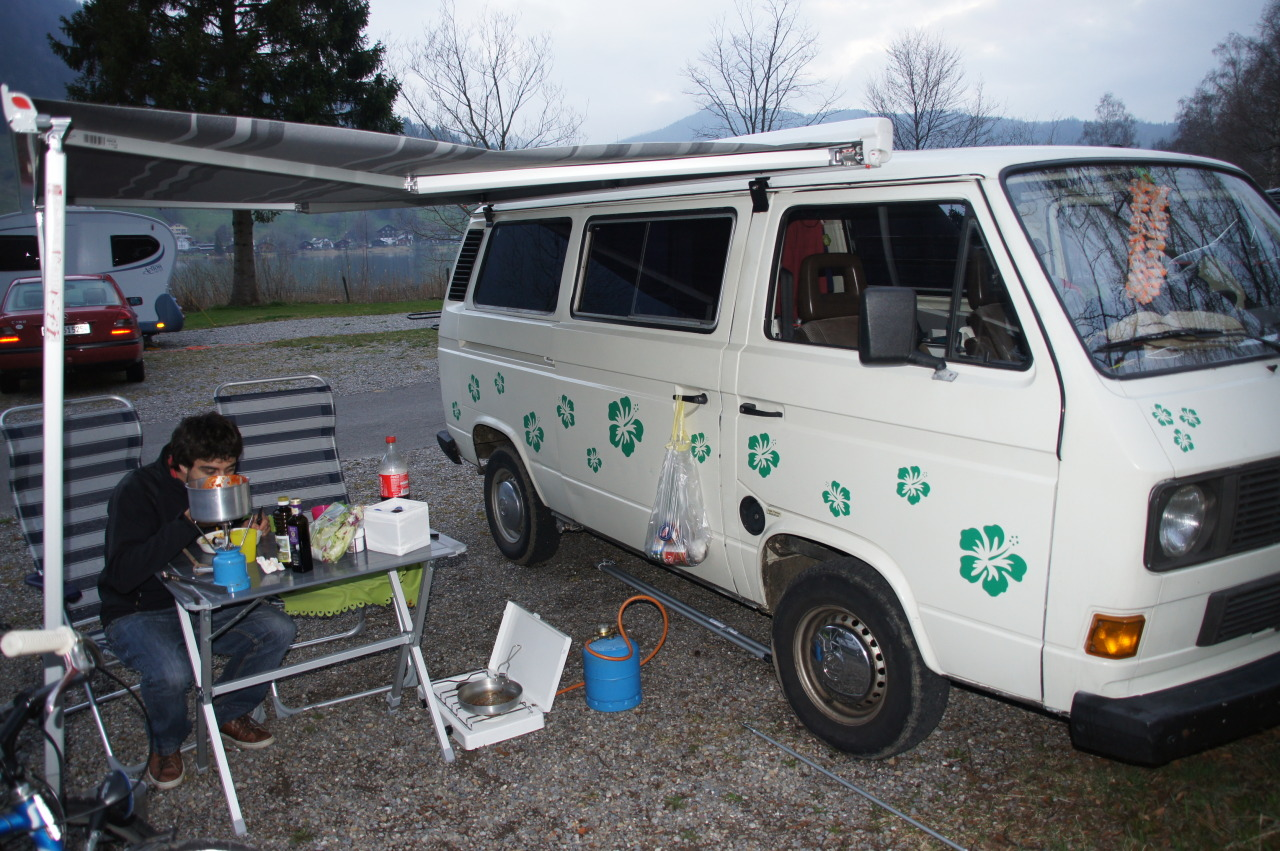
\includegraphics [width=0.3\textwidth]{../Bilder/Aegeri/4.jpg}}\quad
   \subfloat{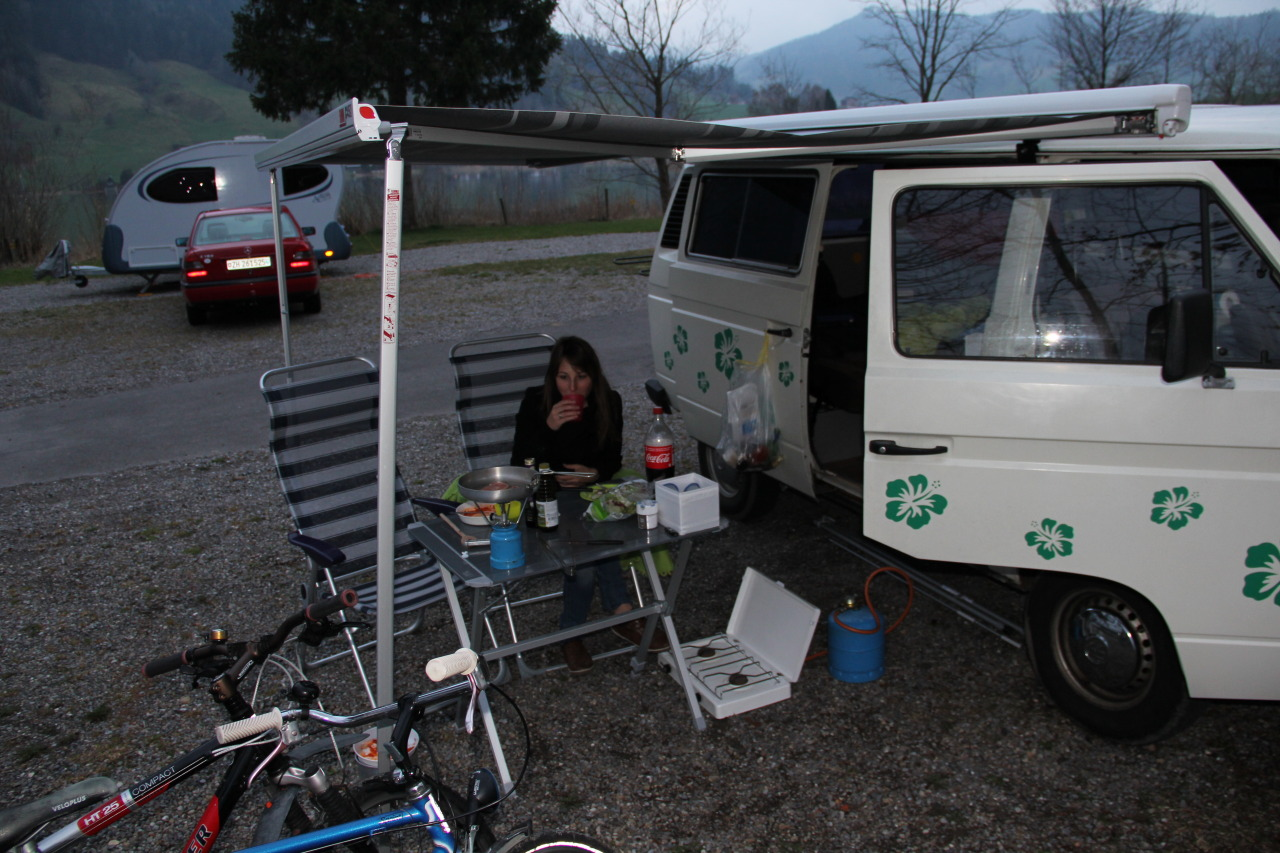
\includegraphics [width=0.3\textwidth]{../Bilder/Aegeri/7.jpg}}\quad
   \caption[Auf dem Campingplatz]{Auf dem Campingplatz}
\end{figure}

\subsection{Samstag 07.04.2012}
Der Samstag zeigte sich vom Wetter her leider noch trister.
Es regnete sehr stark und wir beschlossen noch ein wenig länger liegen zu bleiben.
Zuerst wollten wir mit den ÖV richtig Zug aufbrechen.
Die Wassermassen die vom Himmel fielen, überzeugten uns jedoch bald den VW-Bus zu nehmen.
Nach einem ausgewogenen Frühstück im Bus mussten wir uns auf den Weg machen, da wir sonst bei der Ausfahrt die so heilige Mittagsruhe auf dem Campingplatz verletzt hätten.

\begin{figure}[t]
    \centering
    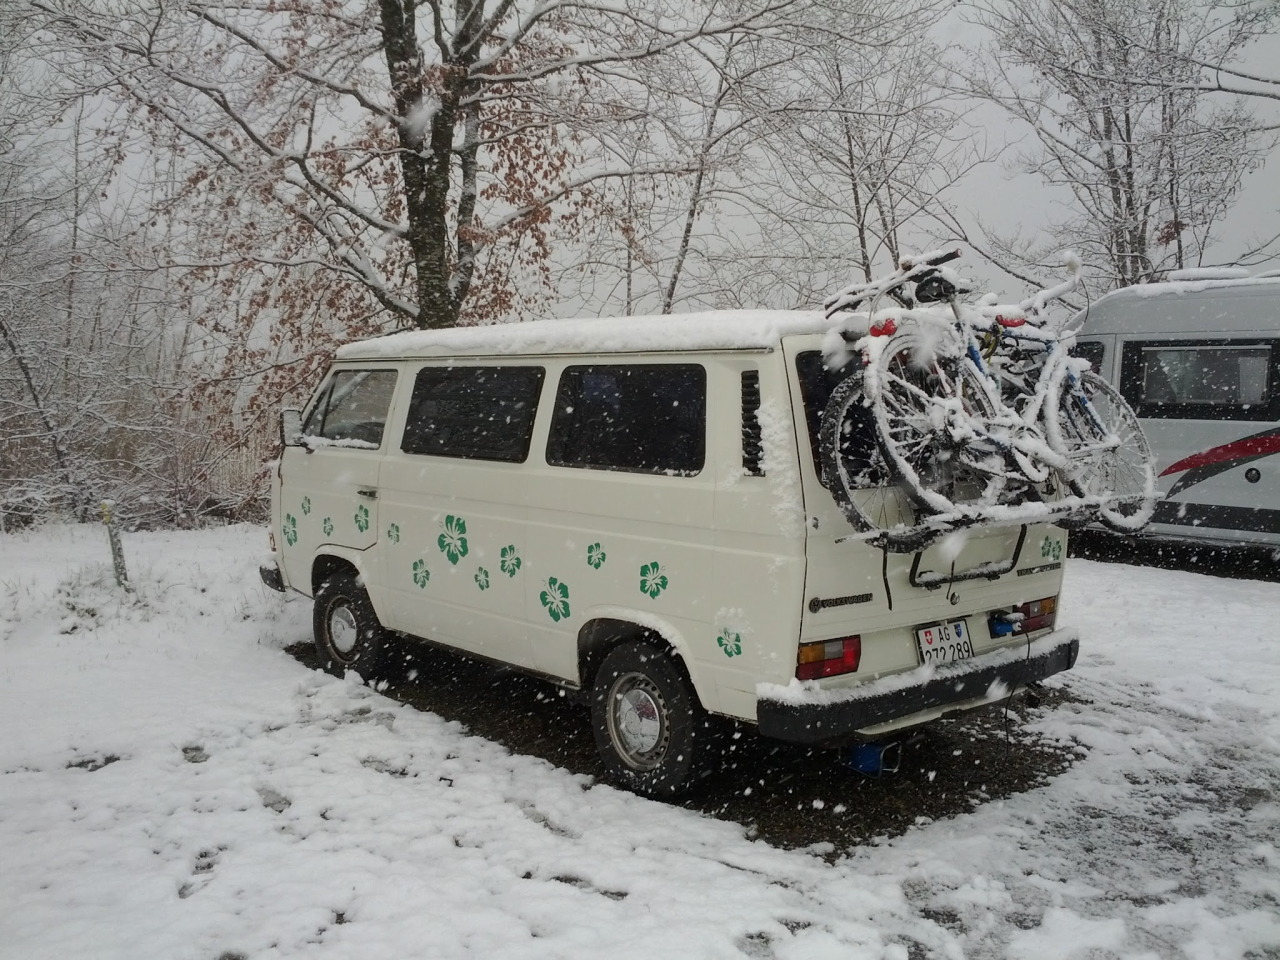
\includegraphics[width=\textwidth]{../Bilder/Aegeri/11.jpg}
    \caption{Vom Winter eingeholt...}
    \label{img:Aegeri}
\end{figure}

Das Parkhaus war schnell gefunden worden und wir machten uns auf, Zug shoppingtechnisch zu erkunden.
Eher eine Qualität, welche Chantal mit sich bringt.
Nach etlichen abgeklapperten Shops und eingelegten Trinkpausen war da ein leichtes Ziehen in der Magengegend zu verspüren.
Dieses äusserste sich bald etwas heftiger bei Chantal und wuchs schnell einmal zu einem Verlangen nach fester Nahrung an.
Blöderweise war es Mitten am Nachmittag an einem Ostersamstag.
Die Frage nach warmen Essen am Nachmittag, welche in einer Pizzeria gestellt wurde, ist zwar positiv beantwortet worden.
Die eingeschränkte Karte konnte Chantal jedoch nicht überzeugen und so reservierten wir einen Tisch um 18:00 Uhr.
Fast zwei Stunden mussten wir noch überstehen und das, nachdem der intensive Pizzageruch meinen Kohldampf wieder geweckt hat.

Nach einem Besuch der Burg und einem kleinen Apéro, begaben wir uns ins Restaurant und genossen ein herrliches Nachtessen.
Den restlichen Abend verbrachten wir mit der Suche meines Autoschlüssels und Witzen was das Wetter noch alles bringen wird.

\subsection{Rückfahrt}
Schön! Kein Getropfe zu hören.
Nur das ratternde Geräusch des Öfelis.
Es hat aufgehört zu regnen.
Tatsächlich regnete es nicht mehr.
Es hat angefangen zu schneien!! Unsere Markise ächzte schon unter der weissen Pracht.
Tapfer entstieg ich dem warmen Auto und befreite todesmutig den arg gebeutelten Stoff von seiner Last.
Nach dem Aufräumen und Morgenessen war uns die Lust am Campen eher vergangen und machten uns auf den Rückweg anzutreten.
Unterwegs wollten wir uns noch die Höllgrotte zu Gemüte führen.
Richtiggehend warm war es da drin.
Eine interessante Erfahrung, durch die mit LED Licht beleuchteten Höhlen zu streifen.
Es wurden kräftig Fotos gesammelt.

\begin{figure}[H]
   \centering
      %\subfloat[CAPTION]{BILDERCODE}\qquad
   \subfloat{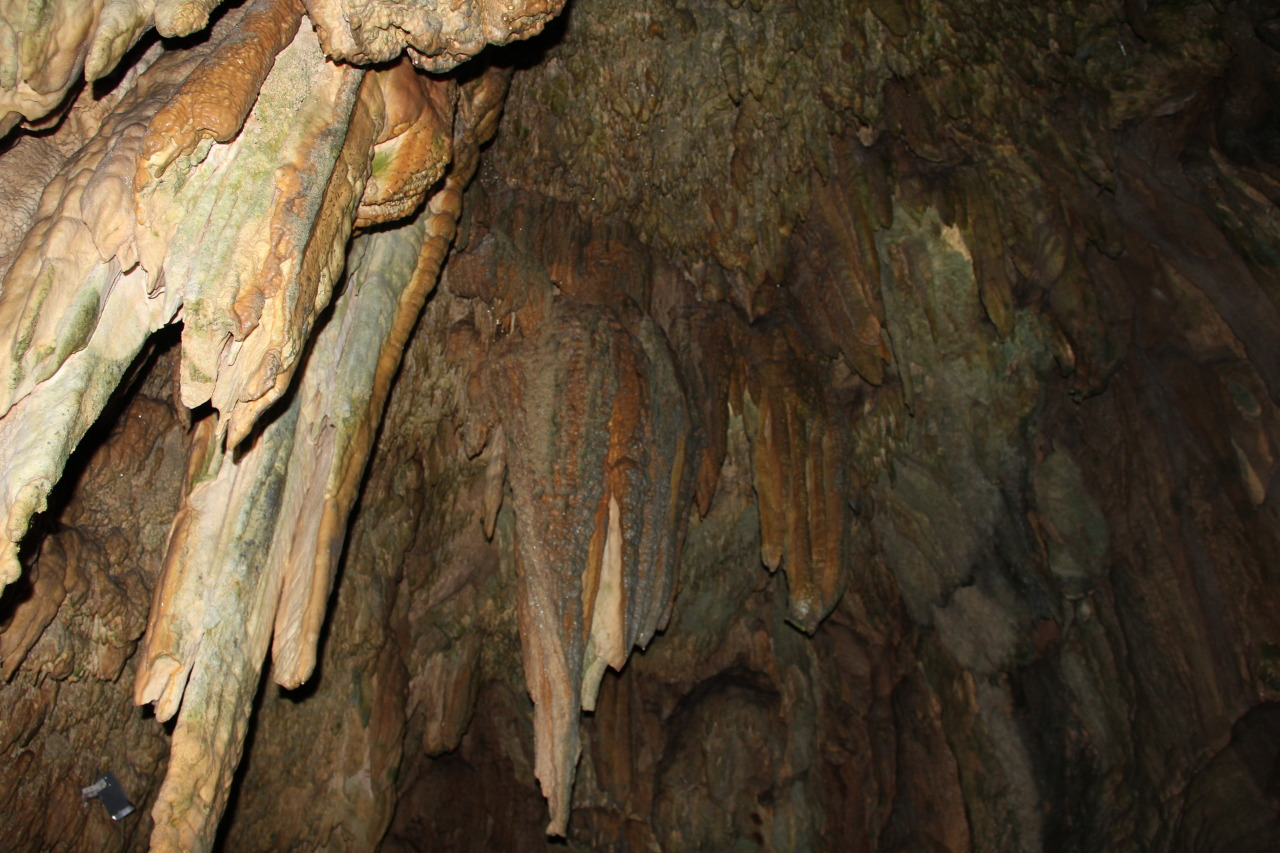
\includegraphics [width=0.3\textwidth]{../Bilder/Aegeri/16.jpg}}\quad
   \subfloat{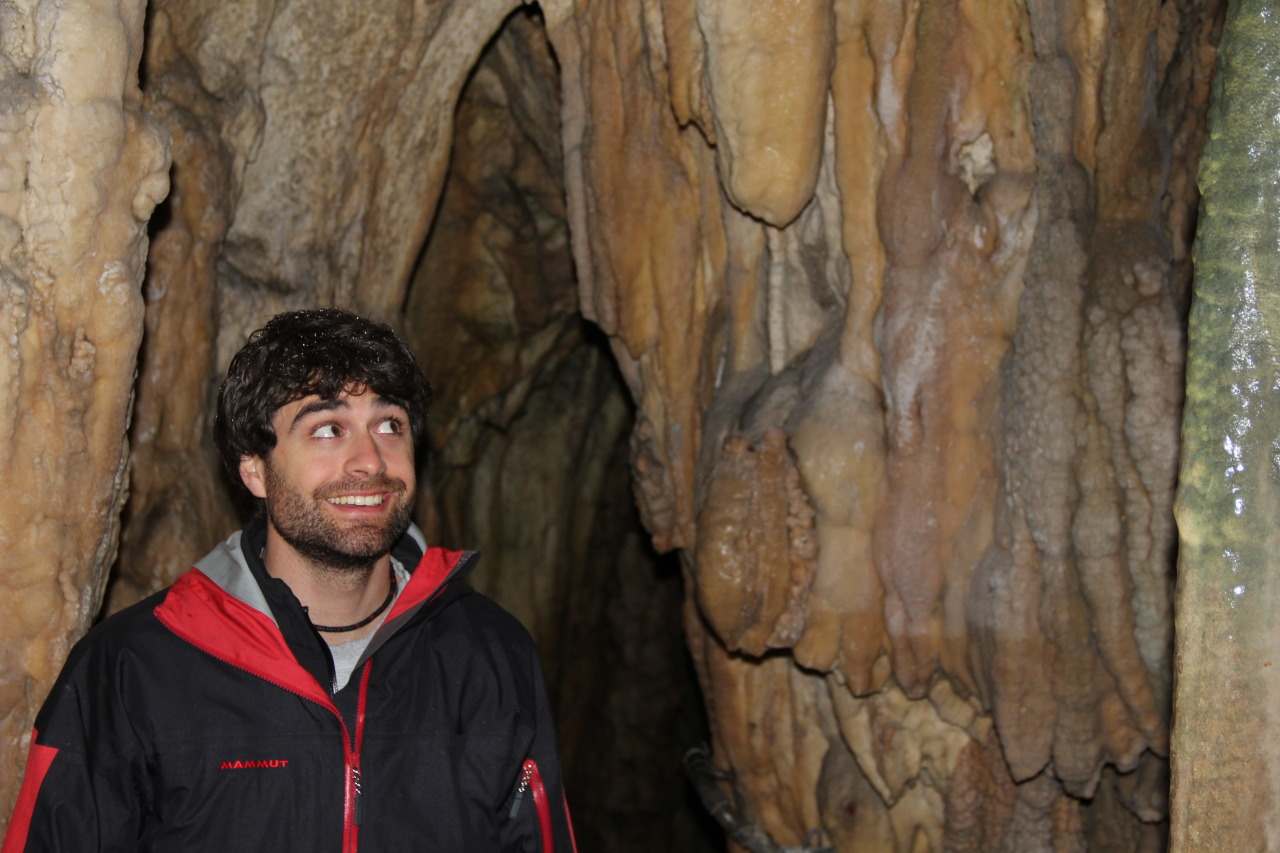
\includegraphics [width=0.3\textwidth]{../Bilder/Aegeri/18.jpg}}\quad
   \subfloat{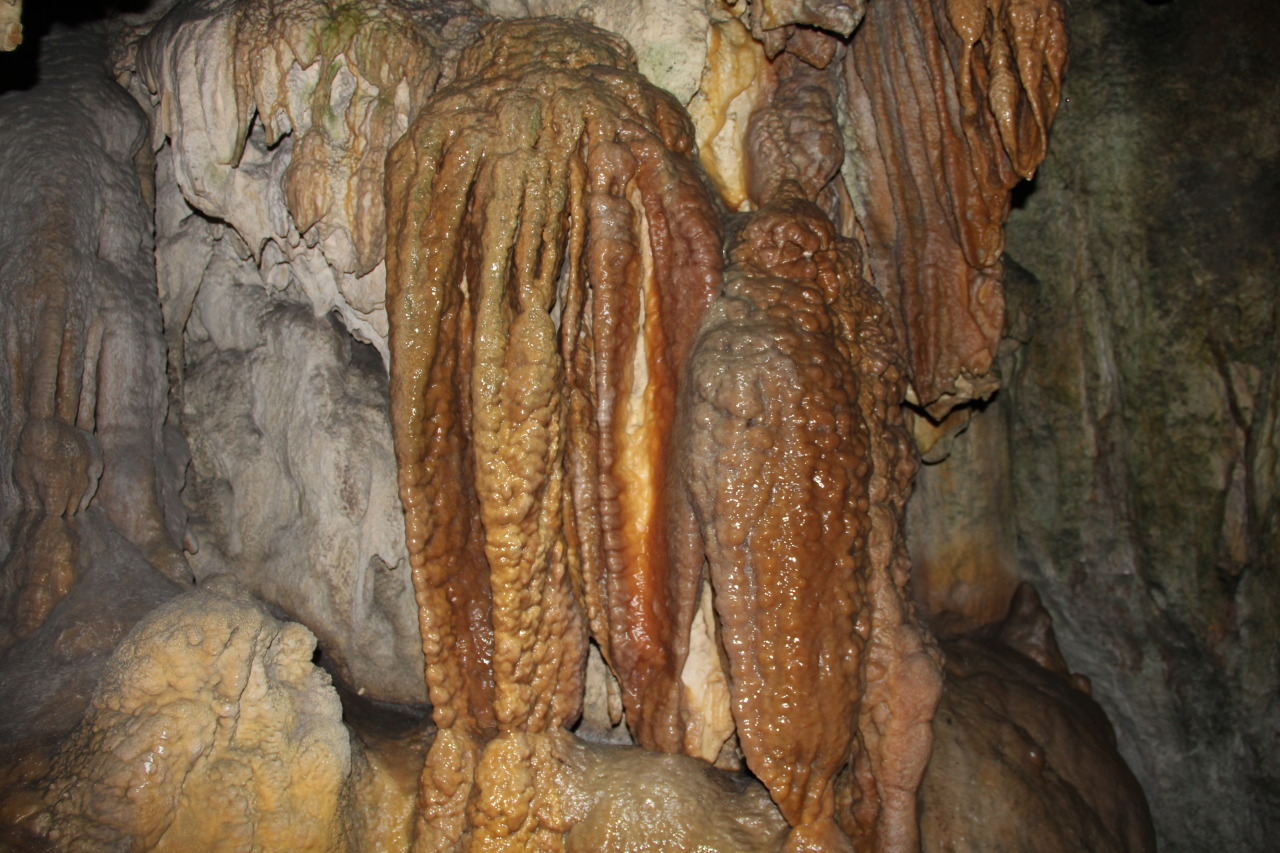
\includegraphics [width=0.3\textwidth]{../Bilder/Aegeri/23.jpg}}\quad
   \caption[In der Höllgrotte]{In der Höllgrotte}
\end{figure}

Die Fahrt zurück nach Hause verlief reibungsfrei aber immer noch bei starkem Schneefall.
Ein Wochenende welches uns unerwartet kaltes Wetter gebracht hat.
Eine spannende Erfahrung, welche wir jedoch noch so gerne mit 20°C Wetter getauscht hätten.
